\documentclass[aspectratio=169,11pt]{beamer}

\usetheme{Madrid}
\usecolortheme{seahorse}
\setbeamertemplate{navigation symbols}{}
\setbeamertemplate{footline}[frame number]
\setbeamertemplate{caption}[numbered]

\usepackage{amsmath}
\usepackage{amssymb}
\usepackage{booktabs}
\usepackage{graphicx}
\usepackage{mathtools}

\title[Viscous Burgers' Equation]{Question 4: Numerical Study of the Burgers' Equation}
\subtitle{Travelling waves, CNLF finite differences, and Chebyshev collocation}
\author{Rishabh Kumar}
\institute{MH7007 Topics in Scientific Computation I}
\date{\today}

\begin{document}

\begin{frame}
    \titlepage
\end{frame}

\begin{frame}{Question 4: Problem Statement}
    We study the viscous Burgers' equation
    \begin{equation}
        u_t+u u_x=\varepsilon u_{xx},
        \qquad x\in\mathbb{R},\quad t>0,\quad \varepsilon>0.
    \end{equation}

    The assignment asks us to:
    \begin{enumerate}
        \item verify the exact travelling-wave solution;
        \item formulate and test a Crank--Nicolson--Leap-Frog (CNLF) finite-difference method;
        \item solve the interval problem on $(-1,1)$ using CNLF in time and Chebyshev collocation in space.
    \end{enumerate}

    \vspace{0.3cm}
    Conservative form will be central:
    \begin{equation}
        u_t+\frac12(u^2)_x=\varepsilon u_{xx}.
    \end{equation}
\end{frame}

\begin{frame}{Part 1: Travelling-Wave Ansatz}
    The proposed solution is
    \begin{equation}
        u(x,t)=\omega\left(1-\tanh\left[
        \frac{\omega}{2\varepsilon}(x-\omega t-x_0)
        \right]\right).
    \end{equation}

    Let
    \begin{equation}
        y=x-\omega t-x_0,
        \qquad u(x,t)=w(y).
    \end{equation}
    Then
    \begin{equation}
        u_t=-\omega w',
        \qquad u_x=w',
        \qquad u_{xx}=w''.
    \end{equation}

    Substitution into Burgers' equation gives
    \begin{equation}
        -\omega w'+w w'=\varepsilon w''
        \quad\Longleftrightarrow\quad
        -\omega w'+\left(\frac{w^2}{2}\right)'=\varepsilon w''.
    \end{equation}
\end{frame}

\begin{frame}{First Integral and Separable ODE}
    Integrating once in $y$,
    \begin{equation}
        -\omega w+\frac{w^2}{2}=\varepsilon w'+C.
    \end{equation}

    For a travelling front with
    \begin{equation}
        w(-\infty)=2\omega,\qquad w(+\infty)=0,\qquad w'(\pm\infty)=0,
    \end{equation}
    we obtain $C=0$. Hence
    \begin{equation}
        \varepsilon w'
        =
        -\omega w+\frac{w^2}{2}
        =
        \frac{w(w-2\omega)}{2}.
    \end{equation}

    Separating variables,
    \begin{equation}
        \frac{dw}{w(w-2\omega)}=\frac{dy}{2\varepsilon}.
    \end{equation}
\end{frame}

\begin{frame}{Solving the Travelling-Wave ODE}
    Using partial fractions,
    \begin{equation}
        \frac{1}{2\omega}
        \int\left(\frac{1}{w-2\omega}-\frac{1}{w}\right)\,dw
        =
        \frac{y}{2\varepsilon}.
    \end{equation}

    Absorbing the integration constant into $x_0$ gives
    \begin{equation}
        w(y)=\frac{2\omega}{1+\exp(\omega y/\varepsilon)}.
    \end{equation}

    Since
    \begin{equation}
        \frac{2}{1+e^A}=1-\tanh\left(\frac{A}{2}\right),
    \end{equation}
    we get
    \begin{equation}
        \boxed{
        u(x,t)=\omega\left(1-\tanh\left[
        \frac{\omega}{2\varepsilon}(x-\omega t-x_0)
        \right]\right).}
    \end{equation}
\end{frame}

\begin{frame}{Direct Verification}
    Define
    \begin{equation}
        \eta=\frac{\omega}{2\varepsilon}(x-\omega t-x_0),
        \qquad
        u=\omega(1-\tanh\eta).
    \end{equation}

    Since $\eta_x=\omega/(2\varepsilon)$ and $\eta_t=-\omega^2/(2\varepsilon)$,
    \begin{align}
        u_x&=-\frac{\omega^2}{2\varepsilon}\operatorname{sech}^2\eta,\\
        u_t&=\frac{\omega^3}{2\varepsilon}\operatorname{sech}^2\eta,\\
        u_{xx}&=\frac{\omega^3}{2\varepsilon^2}
        \operatorname{sech}^2\eta\,\tanh\eta.
    \end{align}

    Thus
    \begin{equation}
        u_t+u u_x
        =
        \frac{\omega^3}{2\varepsilon}
        \operatorname{sech}^2\eta\,\tanh\eta
        =
        \varepsilon u_{xx}.
    \end{equation}
\end{frame}

\begin{frame}{Part 2: Conservative Form and CNLF Grid}
    Use
    \begin{equation}
        u_t+\frac12(u^2)_x=\varepsilon u_{xx}.
    \end{equation}

    Let
    \begin{equation}
        x_m=x_L+mh,\qquad t_n=nk,\qquad V_m^n\approx u(x_m,t_n).
    \end{equation}

    Discretize:
    \begin{align}
        u_t(x_m,t_n)
        &\approx \frac{V_m^{n+1}-V_m^{n-1}}{2k},\\
        \frac12(u^2)_x(x_m,t_n)
        &\approx
        \frac{(V_{m+1}^n)^2-(V_{m-1}^n)^2}{4h},\\
        u_{xx}(x_m,t_n)
        &\approx
        \frac{\delta_x^2V_m^{n+1}+\delta_x^2V_m^{n-1}}{2h^2}.
    \end{align}
\end{frame}

\begin{frame}{CNLF Scheme}
    Here
    \begin{equation}
        \delta_x^2V_m^n=V_{m+1}^n-2V_m^n+V_{m-1}^n.
    \end{equation}

    Substituting into the PDE gives
    \begin{equation}
        \frac{V_m^{n+1}-V_m^{n-1}}{2k}
        +
        \frac{(V_{m+1}^n)^2-(V_{m-1}^n)^2}{4h}
        =
        \frac{\varepsilon}{2h^2}
        \left(\delta_x^2V_m^{n+1}+\delta_x^2V_m^{n-1}\right).
    \end{equation}

    With $\mu=\varepsilon k/h^2$,
    \begin{equation}
        \boxed{
        V_m^{n+1}-\mu\delta_x^2V_m^{n+1}
        =
        V_m^{n-1}+\mu\delta_x^2V_m^{n-1}
        -
        \frac{k}{2h}
        \left((V_{m+1}^n)^2-(V_{m-1}^n)^2\right).}
    \end{equation}
\end{frame}

\begin{frame}{Why This Is a Linear Solve}
    At time level $n+1$, the nonlinear term is already known because it is evaluated at level $n$.

    \begin{block}{Structure}
        \begin{itemize}
            \item Leap-frog in time for $u_t$.
            \item Explicit centered conservative flux for $(u^2)_x/2$.
            \item Crank--Nicolson averaging for the viscous term.
        \end{itemize}
    \end{block}

    Therefore the unknown vector $V^{n+1}$ solves a tridiagonal linear system:
    \begin{equation}
        \left(I-\mu\delta_x^2\right)V^{n+1}=\text{known right-hand side}.
    \end{equation}

    Since CNLF is a two-step method, it requires $V^0$ and $V^1$.
    For the travelling-wave convergence test, $V^1$ is taken from the exact solution.
\end{frame}

\begin{frame}{Local Truncation Error}
    Taylor expansions for a smooth solution give
    \begin{align}
        \frac{u_m^{n+1}-u_m^{n-1}}{2k}
        &=
        u_t+\frac{k^2}{6}u_{ttt}+O(k^4),\\
        \frac{(u_{m+1}^n)^2-(u_{m-1}^n)^2}{4h}
        &=
        \frac12(u^2)_x+\frac{h^2}{12}(u^2)_{xxx}+O(h^4),\\
        \frac{\delta_x^2u_m^{n+1}+\delta_x^2u_m^{n-1}}{2h^2}
        &=
        u_{xx}+\frac{k^2}{2}u_{xxtt}
        +\frac{h^2}{12}u_{xxxx}
        +O(k^4+k^2h^2+h^4).
    \end{align}

    Hence
    \begin{equation}
        \tau_m^n=O(k^2+h^2).
    \end{equation}
\end{frame}

\begin{frame}{Travelling-Wave Numerical Test}
    \small
    Parameters:
    \begin{equation}
        \omega=0.5,\quad
        \varepsilon=0.1,\quad
        x_0=3,\quad
        -5\le x\le 5,\quad
        T=2,\quad
        h=k=10^{-3}.
    \end{equation}

    Notebook result:
    \begin{equation}
        \|e(T)\|_{\infty}=4.548\times10^{-7}.
    \end{equation}

    \begin{figure}
        \centering
        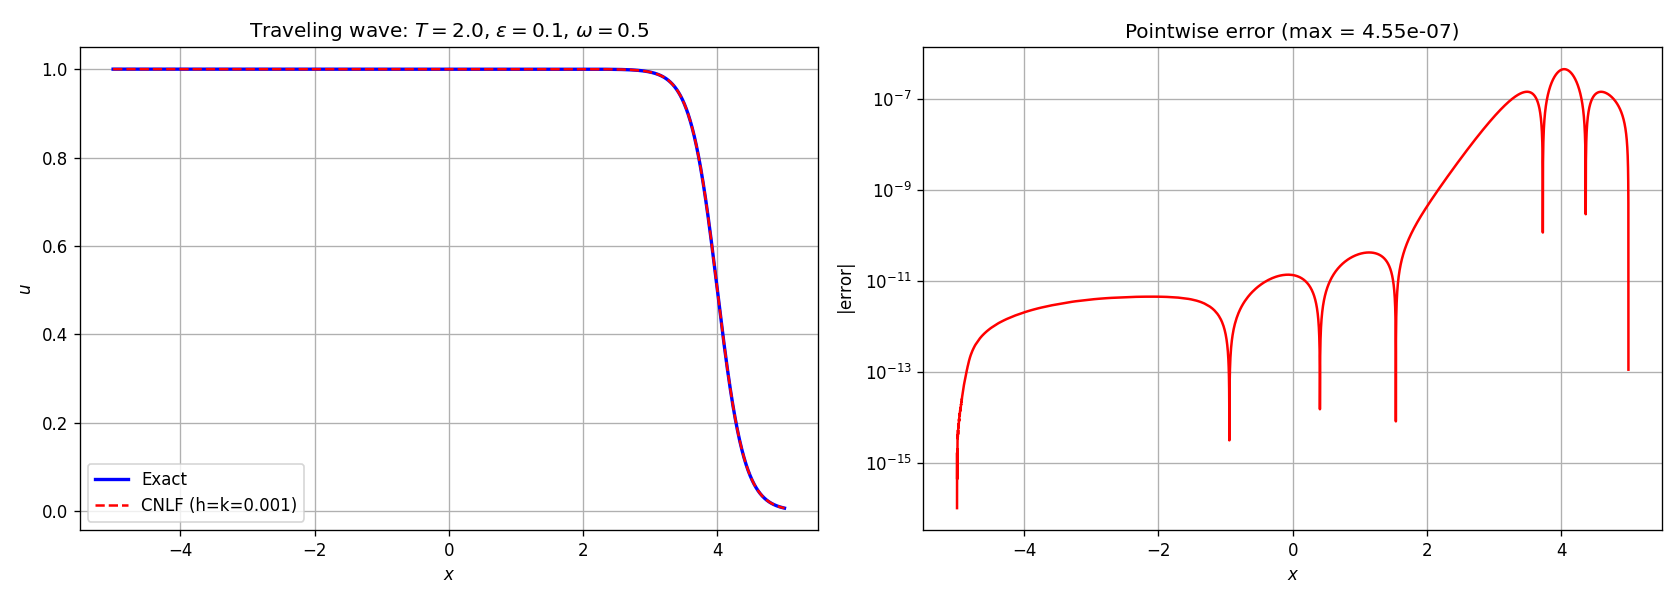
\includegraphics[width=0.72\textwidth]{figures/traveling_wave.png}
    \end{figure}
\end{frame}

\begin{frame}{Coupled Convergence: $h=k$}
    \scriptsize
    \begin{table}
        \centering
        \begin{tabular}{@{}ccc@{}}
            \toprule
            $h=k$ & $\|e(T)\|_\infty$ & rate \\
            \midrule
            0.0400 & $6.056\times10^{-4}$ & -- \\
            0.0200 & $1.513\times10^{-4}$ & 2.001 \\
            0.0100 & $3.790\times10^{-5}$ & 1.997 \\
            0.0050 & $9.485\times10^{-6}$ & 1.998 \\
            \bottomrule
        \end{tabular}
    \end{table}

    \begin{figure}
        \centering
        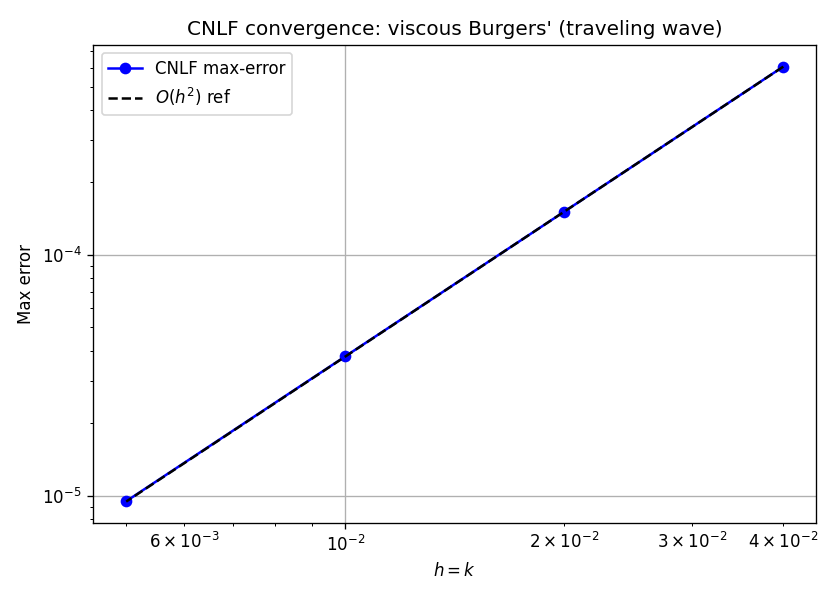
\includegraphics[width=0.38\textwidth]{figures/burgers_convergence.png}
    \end{figure}
    \vspace{-0.35cm}
    \centering The observed slope is second order.
\end{frame}

\begin{frame}{Separate Time and Space Convergence}
    \begin{columns}[T]
        \begin{column}{0.48\textwidth}
            \textbf{Temporal convergence}\\
            $h=2.5\times10^{-4}$
            \begin{table}
                \scriptsize
                \begin{tabular}{@{}ccc@{}}
                    \toprule
                    $k$ & $\|e\|_2$ & rate \\
                    \midrule
                    $8.0\cdot10^{-3}$ & $3.663\cdot10^{-6}$ & -- \\
                    $4.0\cdot10^{-3}$ & $9.125\cdot10^{-7}$ & 2.005 \\
                    $2.0\cdot10^{-3}$ & $2.250\cdot10^{-7}$ & 2.020 \\
                    $1.0\cdot10^{-3}$ & $5.316\cdot10^{-8}$ & 2.081 \\
                    \bottomrule
                \end{tabular}
            \end{table}
        \end{column}
        \begin{column}{0.48\textwidth}
            \textbf{Spatial convergence}\\
            $k=10^{-4}$
            \begin{table}
                \scriptsize
                \begin{tabular}{@{}ccc@{}}
                    \toprule
                    $h$ & $\|e\|_2$ & rate \\
                    \midrule
                    $4.0\cdot10^{-2}$ & $1.584\cdot10^{-4}$ & -- \\
                    $2.0\cdot10^{-2}$ & $3.963\cdot10^{-5}$ & 1.999 \\
                    $1.0\cdot10^{-2}$ & $9.911\cdot10^{-6}$ & 1.999 \\
                    $5.0\cdot10^{-3}$ & $2.478\cdot10^{-6}$ & 2.000 \\
                    \bottomrule
                \end{tabular}
            \end{table}
        \end{column}
    \end{columns}

    \vspace{0.15cm}
    Both experiments confirm $O(k^2)$ and $O(h^2)$ behaviour.
\end{frame}

\begin{frame}{Part 3: Interval Problem}
    Now solve Burgers' equation on $(-1,1)$:
    \begin{equation}
        u_t+u u_x=\varepsilon u_{xx},
        \qquad -1<x<1,\quad t>0,
    \end{equation}
    with
    \begin{equation}
        u(\pm1,t)=0,\qquad
        u(x,0)=-\sin(\pi x),\qquad
        \varepsilon=0.02,\qquad
        T=0.995.
    \end{equation}

    \begin{block}{Spectral collocation choice}
        Fourier collocation is natural for periodic domains. For a nonperiodic interval, the corresponding standard spectral collocation method is Chebyshev collocation.
    \end{block}
\end{frame}

\begin{frame}{Chebyshev--Lobatto Grid}
    Use the Chebyshev--Lobatto points
    \begin{equation}
        x_j=\cos\left(\frac{j\pi}{N}\right),
        \qquad j=0,\ldots,N.
    \end{equation}

    These nodes cluster near $x=\pm1$, helping resolve boundary layers and steep gradients.

    For nodal values $U_j(t)\approx u(x_j,t)$,
    \begin{equation}
        p_N'(x_i)\approx\sum_{j=0}^N D_{ij}U_j.
    \end{equation}

    For $i\neq j$,
    \begin{equation}
        D_{ij}=
        \frac{c_i}{c_j}
        \frac{(-1)^{i+j}}{x_i-x_j},
        \qquad
        c_0=c_N=2,\quad c_j=1.
    \end{equation}
    The diagonal is chosen by $D_{ii}=-\sum_{j\neq i}D_{ij}$, and $D^{(2)}=D^2$.
\end{frame}

\begin{frame}{Chebyshev Semi-Discrete Burgers System}
    In conservative form,
    \begin{equation}
        \dot U+\frac12D(U\odot U)=\varepsilon D^2U,
    \end{equation}
    where $\odot$ denotes componentwise multiplication.

    Impose the Dirichlet conditions:
    \begin{equation}
        U_0=U_N=0.
    \end{equation}

    On the interior nodes $I=\{1,\ldots,N-1\}$, the CNLF update is
    \begin{equation}
        (I-\varepsilon kD^2_{II})U_I^{n+1}
        =
        U_I^{n-1}
        +\varepsilon k(D^2U^{n-1})_I
        -\frac{k}{2}\left(D((U^n)^2)\right)_I.
    \end{equation}
\end{frame}

\begin{frame}{Chebyshev Startup Step}
    Since CNLF is a two-step method, compute $U^1$ from a nonlinear Crank--Nicolson startup:
    \begin{equation}
        U^1-U^0
        +\frac{k}{4}D\left((U^1)^2+(U^0)^2\right)
        -\frac{\varepsilon k}{2}D^2(U^1+U^0)=0.
    \end{equation}

    This nonlinear system is solved by Newton's method on the interior nodes.

    Parameters used:
    \begin{equation}
        N=96,\qquad k=10^{-3},\qquad
        \varepsilon=0.02,\qquad T=0.995.
    \end{equation}
\end{frame}

\begin{frame}{Chebyshev-Collocation Result}
    \begin{figure}
        \centering
        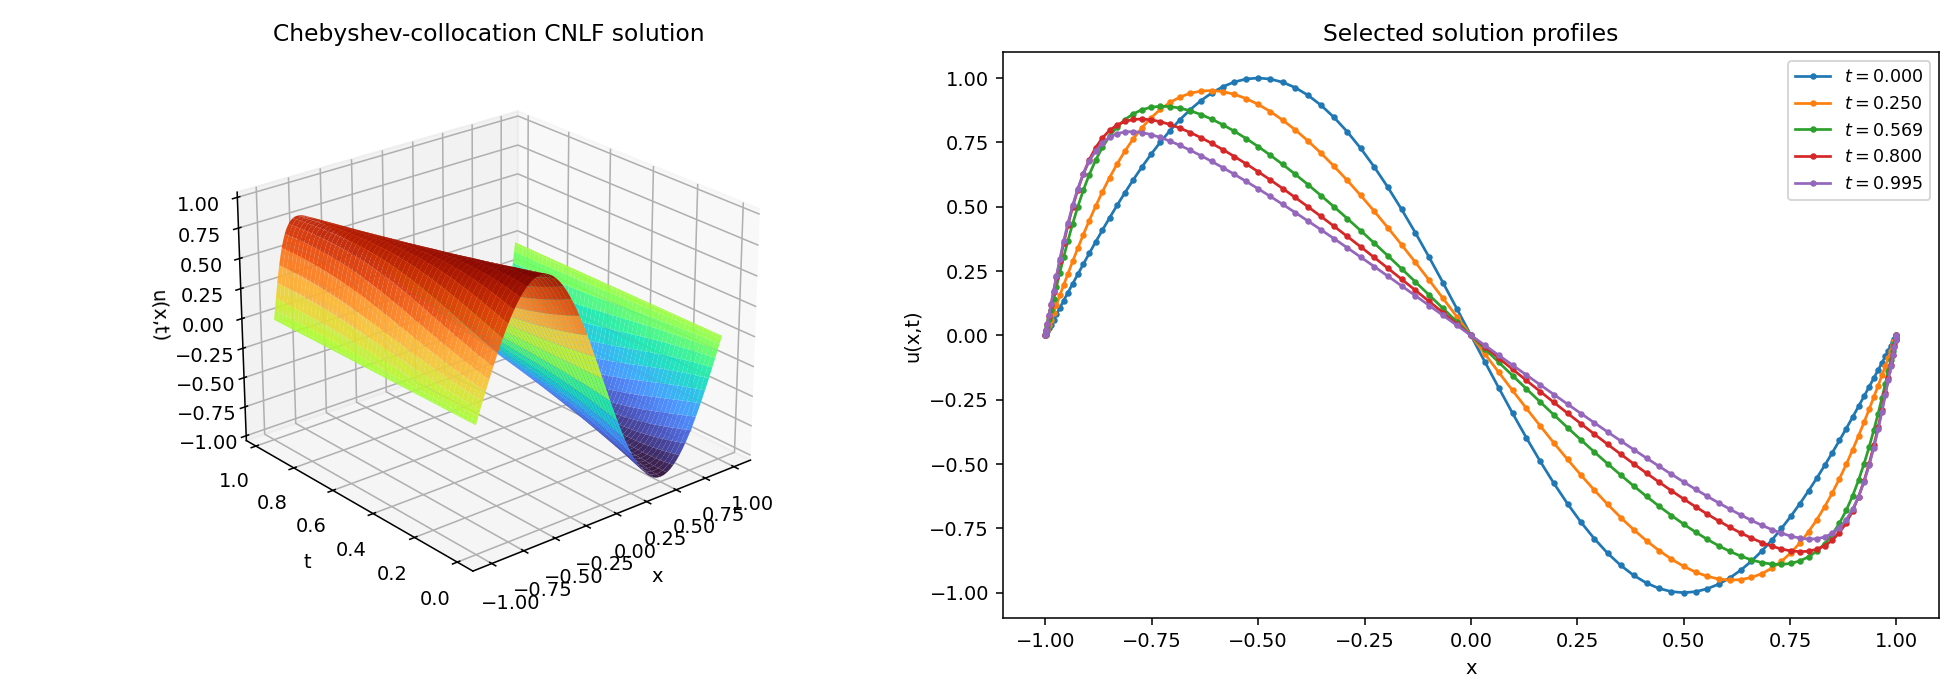
\includegraphics[width=0.88\textwidth]{figures/chebyshev_collocation.png}
        \caption{Chebyshev-collocation CNLF solution and selected profiles.}
    \end{figure}
\end{frame}

\begin{frame}{Finite-Difference Reference Profiles}
    \begin{figure}
        \centering
        
\includegraphics[width=0.58\textwidth]{figures/burgers_sine.png}
    \end{figure}

    \small
    The Chebyshev method captures the same steepening and viscous smoothing with a spectral spatial discretisation.
\end{frame}

\begin{frame}{Takeaways}
    \begin{itemize}
        \item The tanh travelling wave is obtained by a travelling-wave reduction and satisfies Burgers' equation exactly.
        \item Conservative form gives a clean finite-difference approximation of the nonlinear term.
        \item The CNLF method combines leap-frog time stepping, explicit centered flux, and Crank--Nicolson diffusion.
        \item Taylor expansion gives local truncation error $O(k^2+h^2)$.
        \item Numerical tests confirm second-order accuracy.
        \item Chebyshev collocation is the standard spectral alternative for the nonperiodic interval problem.
    \end{itemize}
\end{frame}

\end{document}
